
\documentclass[12pt,a4paper]{article}   % A4 paper, 12pt size font.

%
% Document settings
%
\usepackage{graphicx}          % Allows embedding of most image files.
\usepackage[a4paper]{geometry} % Geometry package for A4 paper.
\geometry{verbose,tmargin=2cm,rmargin=2cm,lmargin=2cm} % Set margins.

\setlength{\parskip}{\bigskipamount}
\setlength{\parindent}{0pt}

\author{Daniel Carrera}
\title{Introduction to MATLAB \\ Practical 1}
\date{2014}

%
% Custom commands.
%
\newcommand{\code}[1]{\texttt{#1}}
\newcommand{\ruler}{
  \begin{center}
    \line(1,0){450}
  \end{center}
}

%
% Main document.
%
\begin{document}

\maketitle

\section{Introduction}

I believe that the best way to learn Matlab is ``\textit{hands on}'', and I tried to
design this practical that way. I assume no prior knowledge of Matlab, but you must
already have it installed. Without further ado, let's start.


\section{Whirlwind tour of MATLAB}

\subsection{Matlab as a calculator}

Locate the Matlab program and run it. After the program starts, you will be presented with
a command shell where you enter Matlab instructions. In the rest of this tutorial,
any line that starts with ``\code{>>}'' denotes the Matlab command shell. For example:

\begin{verbatim}
>> 2 + 3

   5
\end{verbatim}

At the simplest level you can use Matlab as a scientific calculator. Enter the following
code and see what it does.

\begin{verbatim}
>> 2 * 5
>> 2 + 3 * 5 + 1/2
>> 3^2
>> 3^3
>> 3^4
>> 4^(-1)
>> 4^(1/2)
>> sqrt(2)
>> sqrt(4)
>> sqrt(25)
>> pi
>> cos(pi)
>> sin(pi/2)
>> tan(pi/4)
>> atan(1)
>> atan(tan(0))
\end{verbatim}

You can enter arithmetic operations directly into the command window. The symbol \code{\^}
denotes exponentiation (so you write $5^{17}$ as \code{5\^}\code{17}). Matlab has some pre-defined
constants such as \code{pi}, and it supports most standard math functions such as square
roots and trig functions.

\ruler

Enter the following code and see what it does:

\begin{verbatim}
>> exp(0)
>> exp(1)
>> exp(2)
>> e = exp(1)
>> log(e)
>> log(10)
>> log(e^173)
>> log(exp(173))
>> log10(e)
>> log10(10)
>> log10(1000)
>> log10(10^189)
\end{verbatim}

The function \code{exp(x)} returns $e^x$ where $e = 2.7183...$ is the base of the
natural logarithm. The function \texttt{log()} gives the natural logarithm
while \code{log10()} gives the logarithm base 10.

\ruler

Enter the following code and see what it does:

\begin{verbatim}
>> 1i
>> 5i
>> 2 + 1i
>> (-1)^0.5
>> exp(i*pi)
>> log(i)
>> sin(i)
>> sinh(i)
\end{verbatim}

The syntax ``\code{3i}, \code{5i}, etc'' lets you write imaginary numbers safely. Most
operations (exponents, logs, trig) work on complex numbers. \textbf{Do not} use
the variable ``\code{i}'' on its own because it can be overwritten (try \code{i = 7}) and
your program will behave unpredictably.

\ruler

Enter the following code and see what it does:

\begin{verbatim}
>> help log10
\end{verbatim}

Matlab has an extensive help system. I encourage you to use it to learn how functions
work and discover new functions.

\subsection{Vectors and linear algebra}

Enter the following code and see what it does:

\begin{verbatim}
>> u = [1 2 3]
>> v = [3 4 12]
>> u + v
>> u - v
>> 3 * u
>> 3 * u - v
>> dot(u,v)
>> dot(v,v)
>> sqrt( dot(v,v) )
>> norm(v)
\end{verbatim}

One way to create a vector is to enter the vector components directly inside square brackets.
In this example you created row vectors $\vec{u} = [1,2,3]$ and $\vec{v} = [3,4,12]$. You can
do vector addition, subtraction, scalar multiplication and dot product. The function \code{norm} 
returns the norm, or the \textit{magnitude} of a vector.


\ruler

Enter the following code and see what it does:

\begin{verbatim}
>> u
>> v
>> u'
>> v'
>> u' * v
>> u * v'
\end{verbatim}

The vectors \code{u} and \code{v} are row vectors. You need to take the transpose of one
of the vectors to multiply them. An apostrophe denotes matrix transpose, and the \code{*}
operator performs matrix multiplication.


\ruler

Enter the following code and see what it does:

\begin{verbatim}
>> w = [1 ; 2 ; 3 ]
>> w * v
>> v * w
\end{verbatim}

You can also enter a column vector directly if you separate the vector components with
semicolons instead of spaces.


\ruler

\subsection{Conditionals}

Enter the following code and see what it does:

\begin{verbatim}
>> a = 1;
>> b = 2;
>> if a == b
       x = 2;
   elseif a >= 3
       x = 7;
   else
       x = 0;
   end
\end{verbatim}

Experiment with different values of \code{a} and \code{b} and different conditions
(e.g. \code{==  <=  =>  <  >}). What happens if \code{a} and \code{b} are arrays?
Try the following examples:


\begin{verbatim}
>> a = [1 2 3];
>> b = [1 2 3];
>> if a == b
       x = 2;
   else
       x = 0;
   end
>>
>> b = [1 2 4];
>> if a == b
       x = 2;
   else
       x = 0;
   end
>>
>> if any(a == b)
       x = 2;
   else
       x = 0;
   end
>>
>> if all(a == b)
       x = 2;
   else
       x = 0;
   end
>>
\end{verbatim}

Experiment with different arrays (e.g. \code{b = [3 1 2]}). What do the functions
\code{any} and \code{all} do?


\ruler

\subsection{Datasets and plotting}

Notice how the default multiplication operator performs matrix multiplication. In astronomy
we are often more interested in taking two data sets and applying operations term-by-term.
Enter the following code and see what it does:


\begin{verbatim}
>> u = [1 2 3];
>> v = [3 4 12];
>> u .* v
>> u ./ v
>> v ./ u
>> u .^ 2
>> v .^ 2
\end{verbatim}

The operators \code{.*}, \code{./} and \code{.\^} perform \textit{component-wise}
multiplication, division and exponentiation. Notice also that the semicolon at the
end of a line ("\code{;}") causes Matlab to withhold output. When you write longer
programs, you will usually not want to see output for every intermediate step.


\ruler

Enter the following code and see what it does:

\begin{verbatim}
>> 3:11
>> 3:2:11
>> 2.5:7.5
>> 2.5:2:7.5
>> 2:1.5:7
\end{verbatim}


Matlab offers a number of short-cuts for commonly used vectors and matrices. The syntax
\code{a:b} creates a row vector from \code{a} to \code{b} in steps of 1. The syntax
\code{a:q:b} creates a row vector from \code{a} to \code{b} in steps of \code{q}.


\ruler

Enter the following code and see what it does:

\begin{verbatim}
>> x = 1:10;
>> y = x .^ 2;
>> plot(x, y)
>> plot(x, cos(x))
\end{verbatim}

By this point you have learnt enough Matlab to produce many useful plots. Use
\code{x = a:q:b} to create a series of X values, and use vector or array operations
to produce the corresponding Y values. The \code{plot} command is very flexible
and can produce a lot of nice plots.

\ruler

Enter the following code and see what it does. Use the \code{Up} arrow key to pull
up previous lines so that you can save typing:


\begin{verbatim}
>> x = 0:0.1:2*pi;
>> y = sin(x);

>> plot(x,y,'r')
>> plot(x,y,'g')
>> plot(x,y,'b')
>> plot(x,y,'m')
>> plot(x,y,'y')
>> plot(x,y,'k')
>> plot(x,y,'c')

>> plot(x,y,'r-')
>> plot(x,y,'ro')
>> plot(x,y,'r+')
>> plot(x,y,'r*')
>> plot(x,y,'rx')
>> plot(x,y,'r^')

>> plot(x,y,'ro-')
>> plot(x,y,'r+-')
>> plot(x,y,'go-')

>> y2 = cos(x);
>> plot(x,y,'r', x,y2,'b')
>> legend('Sine','Cosine')
>> title('Sines and Cosines')
>> xlabel('This is the X axis')
>> ylabel('This is the Y axis')
\end{verbatim}

The \code{plot} function accepts an optional formatting string to define the colour, plot
style and data label. You can include any number of data sets in the same plot. Run
\code{help plot} to learn more about Matlab's plotting features. Enter the following
program in the Matlab editor:


\ruler

Enter the following code and see what it does:

\begin{verbatim}
>> plot( x, sin(x), 'r' )
>> hold on
>> plot( x, cos(x), 'b' )
>> hold off
\end{verbatim}

The \code{hold on} command causes Matlab to draw any new plotting commands on top of the
existing window. It is one way to draw several data sets on the same plot. The command
\code{hold off} returns Matlab to standard behaviour.

\ruler

\subsection{Making Matlab programs}

Click on the ``New Script'' button to open the built-in Matlab editor. You can
use the editor to write Matlab programs. Matlab programs contain a sequence
of Matlab commands, allowing you to store complex operations fore later use.
When you save the program, the file name must have the extension ``\code{.m}''.
Enter this in the editor:

\begin{verbatim}
% % % % % % % % % % % % % % % %
% 
% wave.m -- An simple animation of a travelling wave.
% 
% % % % % % % % % % % % % % % %

for j = 1:4
    j
end
\end{verbatim}

Save this file as ``\code{wave.m}'' in the current working directory. If the Matlab working
directory is not the same directory that contains the program, Matlab will not be able to
find it. After the file is save, Enter the following in the command window and see what
it does;

\begin{verbatim}
>> wave
\end{verbatim}

This program should print the integers from 1 to 4. This program only contains a short
\textit{for loop}. A \textit{for loop} allows you to repeat commands a fixed number of
times as the index variable (in this case \code{j}) steps through the values of an array.


\ruler

Replace the for loop with the one below and run the program again to see what it does:

\begin{verbatim}
for j = 1.5:0.5:3.5
    j
    j * j
end
\end{verbatim}

The index variable in a for loop can step through the values of any array. The program
also shows Matlab comments. A Matlab comment goes from the \code{\%} sign to the end of
the line. Always comment your programs generously clearly.


\ruler

Update the ``\code{wave.m}'' program with the following one. Run the program and see
what it does:

\begin{verbatim}
% % % % % % % % % % % % % % % %
% 
% wave.m -- An simple animation of a travelling wave.
% 
% % % % % % % % % % % % % % % %

x = 0:0.1:4*pi;  % X values from 0 to 4*pi.
v = -0.1;        % Wave velocity.

for t = 1:1000
    plot( x, sin(x + v*t), 'r' )
    drawnow
    pause(0.2)
end
\end{verbatim}


The \code{drawnow} command causes Matlab to update all figure windows. Without it, the
plot may not be shown until the for loop is complete. The commands \code{sleep} and
\code{usleep} cause Matlab to suspend the program for a given number of seconds (for
\code{sleep}) or microseconds (for \code{usleep}). Without a delay, the for loop may
run too fast.


\ruler

\section{Exercises}

It is important that you do the exercises, as they will help sharpen your skills with
loops, plotting and the Matlab help. The last problem is mainly to help you play with
MATLAB.

\textbf{Exercise 1:} The Fibonacci sequence is a series of integers, starting with ``1,1'', where
the next value is the sum of the previous two values. The first few terms of the Fibonacci
sequence are: ``1,1,2,3,5,8,13,..''. Write a program that prints the first 50 values of the
Fibonacci sequence.

\textbf{Exercise 2:} Try to make a plot similar to the one on the next page. The plot compares the values produced by the \texttt{randn} function with the Gaussian distribution. You will need the following functions: \texttt{hist}, \texttt{randn}, \texttt{normpdf}, \texttt{title}, \texttt{xlabel}, \texttt{ylabel}, \texttt{legend}, \texttt{hold on} and \texttt{hold off}. Use the MATLAB help to figure out what these do.

\begin{figure}[h!]
  \centering
  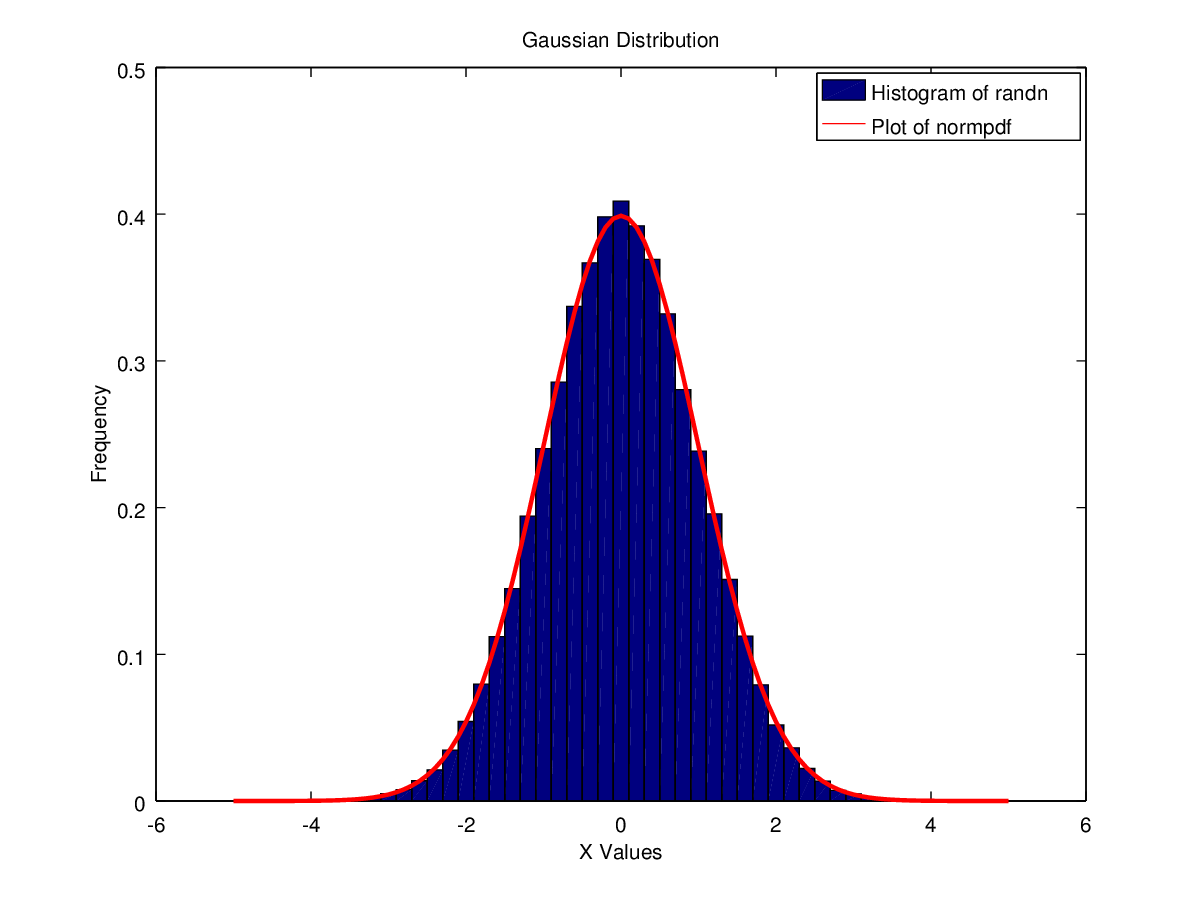
\includegraphics[width=0.7\textwidth]{img/gaussian.png}
\end{figure}


% You will need the following: (1) \texttt{hist} (histograms); (2) \texttt{randn} (normally distributed random values); (3) \texttt{normpdf} (computes Gaussian/normal probabilities); (4) \texttt{title}, \texttt{xlabel}, \texttt{ylabel} and \texttt{legend} (label the plot); and (5)  \texttt{hold on} / \texttt{hold off}. Use the \texttt{help} function to guide you along.


% 
% x = [-5:0.1:5];
% hist( randn(100000,1), [-5:0.2:5], 5 )
% hold on
% plot(x, normpdf(x), 'r-', 'linewidth',2 )
% 
% title("Gaussian Distribution")
% xlabel("X Values")
% ylabel("Frequency")
% 

\textbf{Exercise 3:} Type in the following code and see what it does:

\begin{verbatim}
[x,y] = meshgrid(-8:0.5:8);
r = sqrt(x.^2 + y.^2);
z = sin(r) ./ r;
mesh(x,y,z)
surf(x,y,z)
\end{verbatim}

Use your mouse to grab the image and rotate it, so you can see it from different angles.
Use the help function to learn what \texttt{meshgrid}, \texttt{mesh} and \texttt{surf} do.
Then try to make a plot with an interesting shape (a bowl, a volcano, a sombrero, etc).

\pagebreak


\end{document}





